\documentclass{ctexart}
\usepackage{hyperref}
\hypersetup{
	colorlinks=true,
	linkcolor=black,
	filecolor=blue,      
	urlcolor=blue,
	citecolor=cyan,
}
\usepackage{amsmath}
\usepackage{graphicx}
\usepackage{float}
\usepackage{listings}
\usepackage{xcolor}

\title{基于Vulkan的GPU Driven Rendering教程}
\author{译:fangcun}
\begin{document}
\maketitle
\newpage
\setcounter{tocdepth}{3}
\tableofcontents

\newpage
\section{序}

\subsection{感谢作者}

本文原文:\href{https://vkguide.dev/docs/gpudriven}{链接}

\newpage
\section{GPU Driven Rendering概述}

\begin{figure}[H]
	\title{需要处理125,000个对象,4000万个三角形,仍然达到了290FPS}
	\centering
	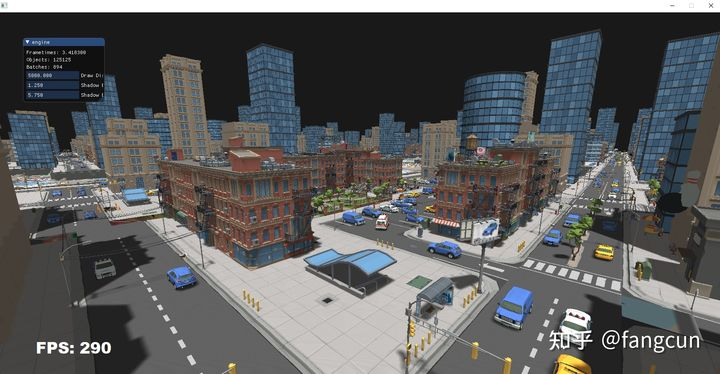
\includegraphics[scale=0.5]{img/1-1.jpg}
\end{figure}


过去几年,人们越来越倾向于在计算着色器中做更多的工作。加之类似MultiDrawIndirect等特性的出现,我们也能够将更多的渲染准备工作放在计算着色器中进行。这样做的好处也有很多:

\begin{itemize}
	\item 对于可以基于数据并行的情况,GPU计算要比CPU计算高效得多。而渲染工作大多数情况下可以基于数据并行。
	\item 不需要在CPU和GPU间进行数据传输,减少了不必要的数据传输延迟。
	\item GPU做了更多的工作,从而解放了CPU的计算能力,这部分CPU的计算能力可以用于其它工作。
\end{itemize}

GPU Driven Rendering可以使我们渲染出更复杂的场景。使用我们的实例代码在Nintendo Switch上可以达到60FPS下,每帧250.000次"drawcall"。在PC上同样次数的"drawcall"可以达到500FPS。我们发现渲染瓶颈由场景中的对象个数变为场景中的三角形个数。

\begin{figure}[H]
	\title{使用了GPU Driven后,CPU计算用时甚至小于0.5毫秒}
	\centering
	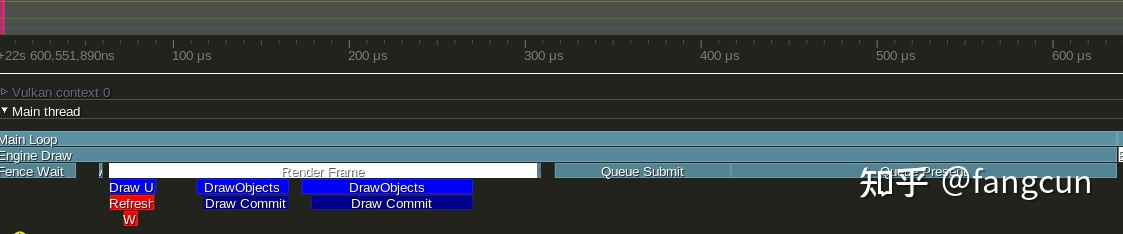
\includegraphics[scale=0.3]{img/1-2.jpg}
\end{figure}

最近5年,使用计算着色器进行渲染计算变得越来越流行。在之前,通常只有CAD软件会更多使用计算着色器。而现在《刺客信条 大革命》使用这一技术让游戏场景的复杂度上了一个台阶。寒霜引擎使用这一技术让游戏《龙腾世纪》有了更多的几何细节。《彩虹6号》使用这一技术让游戏的场景破坏更加真实。因为三角形吞吐量的限制,使用这一技术进行更为精准得剔除操作在PS4和XBox One主机上非常流行。虽然目前UE4和Unity没有使用这一技术,但未来的UE5将会使用它。

\subsection{间接绘制}

GPU Driven Rendering的核心是对图形API提供的间接绘制特性的使用。 虽然大多数图形API都支持间接绘制特性,但Vulkan和DX12因为可以更为细致地进行内存管理,以及计算同步,使用这一特性带来的提升更大。

间接绘制是一个参数来自GPU内存(显存)的drawcall。使用间接绘制时,我们会将一个GPU内存地址传给函数,然后GPU就会按照GPU内存中的参数执行绘制质量。

伪代码如下:

\begin{lstlisting}[language={[ANSI]C},keywordstyle=\color{blue!70},commentstyle=\color{red!50!green!50!blue!50},frame=shadowbox, rulesepcolor=\color{red!20!green!20!blue!20},basicstyle=\small,numbers=left, numberstyle=\tiny,breaklines=true]
//normal drawing ---------------
vkCmdDrawIndexed(cmd, object.indexCount, 1 /* instance count */,object.firstIndex, object.vertexOffset, object.ID /* firstInstance */ );

//indirect drawing ---------------

Buffer* drawBuffer = create_buffer(sizeof(VkDrawIndexedIndirectCommand));

//we can immediately enqueue the draw indirect
vkCmdDrawIndexedIndirect(cmd, drawBuffer.buffer, 0 /* offset */, 1 /* drawCount */, sizeof(VkDrawIndexedIndirectCommand));


//we can write the actual draw command at any time we want before VkQueueSubmit(), or from a different thread, or from a compute shader
VkDrawIndexedIndirectCommand* command = map_buffer(drawBuffer);

command->indexCount = object.indexCount;
command->instanceCount = 1;
command->firstIndex = object.firstIndex ;
command->vertexOffset = object.vertexOffset;
command->firstInstance = object.ID;
\end{lstlisting}

因为绘制的参数来自GPU内存(显存),而计算着色器可以访问到这部分GPU内存(显存),基于这点,我们就可以使用计算着色器来设置绘制指令的参数。我们可以在计算着色器中进行剔除计算,进行LOD层级的选择等等。可以想象对于具有强大并行计算能力的GPU来说,在0.5毫秒内剔除上百万对象是可以做到的,当然,一般情况下也不会有这么复杂的场景。更高级的用法,比如彩虹6号通过写入索引缓冲,实现了使用计算着色器剔除网格中的部分三角形的能力。

对于GPU Driven来说,因为我们想要尽可能地把计算放在GPU上,所以就需要我们更多地把数据放在GPU内存(显存)上,来允许计算着色器访问它们。我们也应该尽量少用Push Constant和基于对象的DescriptorSet,尽量多地避免CPU和GPU间的数据交换。

为了可以访问更多数据,我们可以使用Bindless技术。这一技术使得我们不再需要频繁绑定/解除绑定资源。Doom Eternal的游戏引擎就采用了完全Bindless的方案,将游戏每帧的drawcall降到了非常低的水平。在本教程,我们也会使用Bindless技术,但由于纹理贴图的Bindless支持不太好,导致对于每个不同的材质我们会进行一次间接绘制调用。对于其它部分,比如网格数据,我们会将它合并在一个大的顶点缓冲中,从而避免频繁绑定/解除绑定不同的顶点缓冲。

\subsection{Bindless设计}

\begin{figure}[H]
	\centering
	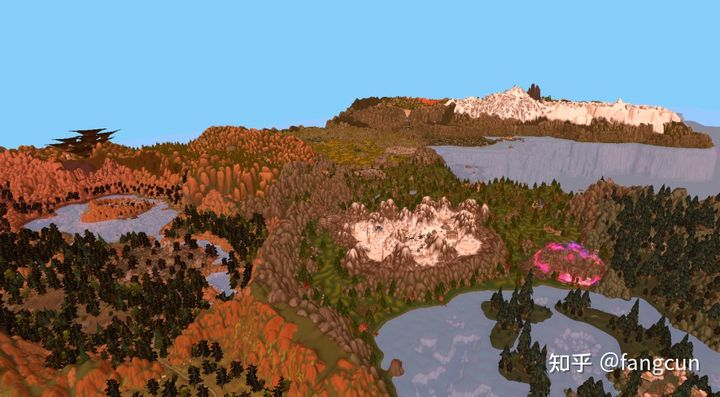
\includegraphics[scale=0.4]{img/1-3.jpg}
\end{figure}

上图仅用10个drawcall以100+FPS的速度实现了大场景渲染。

对于GPU Driven Rendering来说,需要绑定的资源越少,效果越好。也就是说,我们应该尽可能少得进行BindVertexBuffer、BindIndexBuffer、BindPipeline和BindDescriptorSet这类调用。Bindless技术通过让所需得绑定调用变少来减少CPU端所需得工作,从而让CPU端可以跑得更快。GPU端也因为每个"drawcall"的数据量变大,也发挥出了更多的潜力。虽然表面看上去drawcall变少,但GPU的使用率实际上变得更高。

一般来说,我们会将一个场景中的所有网格的顶点缓冲和索引缓冲合并成一个大的数据块来实现顶点缓冲和索引缓冲的Bindless。相比于之前场景中的每个网格对象都有一对顶点缓冲和索引缓冲,渲染不同网格对象不再需要切换顶点缓冲和索引缓冲,只需要修改drawcall中的数据偏移值即可。

目前已经有一些引擎尝试完全不使用顶点属性,直接在着色器中访问GPU内存(显存)来获取顶点数据。通过这种方法让所有drawcall都使用一个大的顶点缓冲变得更加容易,即使这些顶点数据的格式对于不同drawcall可能是不同的。这一方法也使得我们可以使用一些更加高级的数据解压缩方案。

为了实现纹理贴图的Bindless,我们需要使用纹理数组(texture arrays)。通过使用Descriptor Index扩展特性,我们可以做到几乎无限制地在着色器中访问纹理。这一扩展特性允许我们使用GPU内存(显存)中的数据来索引访问纹理。

为了实现材质的Bindless,我们需要将材质参数的设置从管线对象转移到SSBO上,并且采用ubershader技术来尽可能多得减少管线对象的数量。Doom eternal通过这样做,整个游戏只是用了不超过500个管线对象。作为对比的UE引擎做的游戏经常会有100000+的管线对象。因为VkCmdBindPipeline调用的代价很大,通过ubershader技术大量减少管线对象对于性能提升也比较明显。

Push Constants和动态Descriptor虽然也可以使用,但它们设置的数据应该是"全局"的。比如我们可以用Push Constants来设置相机的位置,但对于设置对象ID这样需要每个对象调用一次的情况,就不太适用,这样做我们就没法在一个drawcall绘制多个不同的对象啦。

总的来说,Bindless的基本思想就是尽可能把所有数据都放进一个大的GPU内存(显存),从而避免经常进行绑定/解绑定操作。此外,因为数据都放在了GPU内存中,我们也可以在着色器中很方便地对它们进行修改。龙腾世纪游戏就是通过在着色器中修改缓冲区中的索引数据实现三角形级别的剔除操作。

\subsection{相关资源链接}

\begin{itemize}
	\item 刺客信条 大革命:\href{https://www.advances.realtimerendering.com/s2015/aaltonenhaar_siggraph2015_combined_final_footer_220dpi.pdf}{链接}
	\item 龙腾世纪的网格剔除:\href{https://www.gdcvault.com/play/1023109/Optimizing-the-Graphics-Pipeline-With}{链接}
	\item 彩虹6号:\href{https://www.gdcvault.com/play/1022990/Rendering-Rainbow-Six-Siege}{链接}
	\item Doom:\href{https://advances.realtimerendering.com/s2020/RenderingDoomEternal.pdf}{链接}
	\item 英伟达的高级场景图:\href{https://on-demand.gputechconf.com/gtc/2013/presentations/S3032-Advanced-Scenegraph-Rendering-Pipeline.pdf}{链接}
\end{itemize}

\subsection{本教程示例引擎的架构概述}

我们的示例引擎将所有数据都放在了GPU内存(显存)中,不存对于每个网格对象的PushConstants调用,每个网格对象的动态Uniform缓冲区的更新,所有这些类似操作都被换成了对于某一块GPU内存(显存)的数据更新与访问。

在载入场景时,我们创建一个大的顶点缓冲区,将所有网格数据都放入了这一大的顶点缓冲区中。

完成数据的合并处理后,我们就可以开始实现间接绘制。

\begin{figure}[H]
	\centering
	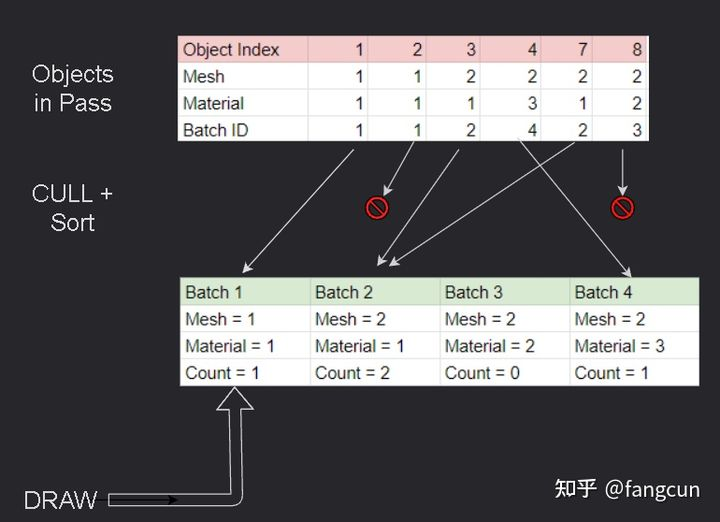
\includegraphics[scale=0.4]{img/1-4.jpg}
\end{figure}

我们将可渲染对象按照mesh pass进行划分。每个mesh pass对应渲染器的一个渲染步骤。对于我们的示例引擎,只有2个mesh pass,一个用于前向渲染网格对象本身,一个用于渲染阴影。可渲染对象可以同时出现在两个mesh pass中,也可以只出现在其中一个(比如某个对象不会产生阴影就不需要出现在绘制阴影的mesh pass)。通过这种mesh pass的划分,可以简化渲染逻辑的实现,也有可能带来更好的性能表现。

我们实现间接绘制的代码可以在RenderScene类中找到,我们首先获取同一个mesh pass中的对象列表,然后将它们划分为不同的批次(batch)。一个批次(batch)中的对象具有相同的材质和网格数据,可以通过一次间接绘制调用进行渲染。每个mesh pass包含了一个用于渲染的批次(batch)数组。

我们将每个对象使用的矩阵数据存储在引擎载入网格对象时生成的用于剔除网格对象的数据旁。

当开始一帧时,我们将每个mesh pass中的对象的ID及其所属批次(batch)的ID放入一个数组中。

当完成数组的数据设置,我们使用计算着色器使用数组中的数据进行对象的剔除。对于数组中的每一个ObjectID+BatchID元素,我们使用它的ObjectID索引访问对象的用于剔除的包围盒数据,检测对象是否可见,如果对象可见,我们使用BatchID索引访问批次数组,将对应批次(batch)的实例数量加1。

当计算着色器的剔除计算完成,我们就可以在CPU端遍历mesh pass对应的批次(batch)数组,绑定对应的管线对象和包含有材质信息的descriptor set。然后就可以使用间接绘制渲染剔除计算后可见的对象。

\newpage
\section{引擎架构概述}

\subsection{代码说明}

读者可以在我们的代码仓库的engine分支找到间接绘制(draw indirect)的所有代码实现:\href{https://github.com/vblanco20-1/vulkan-guide/tree/engine}{代码仓库链接}

这里对仓库中的代码文件进行简要的说明:

\begin{itemize}
	\item imgui支持:我们使用imgui来绘制UI,这部分代码实现主要位于VulkanEngine类中。
	\item CVars.h/cpp:我们实现的用于配置引擎参数的类。
	\item player\_camera.h:我们实现的用于在场景中漫游的相机系统。
	\item logger.h:我们实现的用于输出引擎日志的类。
	\item vk\_pushbuffer:用于向动态descriptor使用的缓冲区更新数据。
	\item vk\_profiler:用于性能分析,统计每个pass的计算耗时,以及统计GPU处理的三角形个数。
	\item vk\_engine\_scenerender.cpp:剔除和绘制指令的逻辑实现。
	\item vk\_scene:实现了对间接绘制所使用的GPU内存(显存)的管理,以及对mesh pass的管理。
	material\_system:材质系统的抽象,包括对管线对象和descriptor的抽象
	\item vk\_descriptors:对descriptor set的抽象。
	\item vk\_shaders:对编译后的shader代码的处理。使用反射自动从编译后的shader代码获取管线布局信息等等。
	\item 资源系统:用于生成引擎可载入的网格数据,生成预制体和材质数据。支持GLTF和FBX文件。预制体是一个包含有场景结点的列表,引擎在载入预制体时可以将其转换为多个可渲染对象。
	\item 计算着色器:计算着色器的相关逻辑位于VulkanEngine类中,主要是计算管线的构造以及用于同步的代码。
\end{itemize}

\subsection{渲染流程}

引擎初始化后,会将一些预制体作为Mesh对象载入场景。场景管理类RenderScene会将这些Mesh对象按照它们的材质信息和配置将它们注册进多个对应的mesh pass。

对于我们的示例引擎,它存在3个mesh pass。一个前向pass,用于渲染不透明对象,一个透明pass,用来渲染半透明对象,最后还有一个阴影pass,用来渲染阴影贴图。Mesh对象在被载入场景时,引擎会按照它的材质信息和配置将它们注册到对应的mesh pass。一般来说,不透明的Mesh对象,会被注册到前向pass和阴影pass,而半透明的对象,一般我们不想让它产生阴影,只会被注册进半透明pass。

一旦场景中的Mesh对象载入完成,RenderScene::build\_batches和RenderScene::merge\_meshes就会被调用。其中build\_batches调用会对所有mesh pass进行处理,生成对应的间接绘制指令。merge\_meshes调用会对场景中的所有网格对象的网格数据进行合并,存储到一个大的顶点缓冲中。

接着,就进入到了帧循环。

在帧循环的开始,我们会清空用于单次帧循环的缓存。然后调用ready\_mesh\_draw函数对变化过的mesh对象的数据进行更新。

等上一步结束后,对于每一个mesh pass,我们就可以调用ready\_cull\_data函数来重置其中每个网格对象的可见状态,等待之后在计算着色器中写入新的可见状态信息。

为了数据的正确同步,我们会使用一个管线barrier来确保上一步的多个ready\_cull\_data调用写入的可见状态信息在计算着色器执行剔除计算前完成。

在计算着色器的剔除计算和渲染绘制指令间,我们也加入了一个管线barrier来保证渲染绘制只会在剔除计算后进行。

对于我们的示例引擎,渲染绘制首先执行shadow\_pass绘制阴影贴图,然后执行前向pass绘制不透明对象,最后执行透明pass,绘制半透明对象。

渲染绘制结束后,我们使用深度缓冲中的数据生成一个多级深度纹理,用于加速下一帧的剔除计算。

最后,我们将场景渲染后的图像放入交换链用于渲染结果的呈现。

\newpage
\section{间接绘制API}

本章节我们主要介绍间接绘制(draw indirect)是如何工作的。

Vulkan提供了下面这两个用于间接绘制(draw indirect)的API:

\begin{lstlisting}[language={[ANSI]C},keywordstyle=\color{blue!70},commentstyle=\color{red!50!green!50!blue!50},frame=shadowbox, rulesepcolor=\color{red!20!green!20!blue!20},basicstyle=\small,numbers=left, numberstyle=\tiny,breaklines=true]
//indexed draw
VKAPI_ATTR void VKAPI_CALL vkCmdDrawIndexedIndirect(
	VkCommandBuffer                             commandBuffer,
	VkBuffer                                    buffer,
	VkDeviceSize                                offset,
	uint32_t                                    drawCount,
	uint32_t                                    stride);

//non indexed draw
VKAPI_ATTR void VKAPI_CALL vkCmdDrawIndirect(
	VkCommandBuffer                             commandBuffer,
	VkBuffer                                    buffer,
	VkDeviceSize                                offset,
	uint32_t                                    drawCount,
	uint32_t                                    stride);
\end{lstlisting}

间接绘制API调用的第一个参数是存储了真正的绘制参数的VkBuffer对象。执行间接绘制,GPU会从指定的VkBuffer对象的offset+(stride * index)处读取出真正的绘制参数,然后进行绘制,整个过程重复drawCount次。下面的代码给出了真实的绘制参数在内存中的布局:

\begin{lstlisting}[language={[ANSI]C},keywordstyle=\color{blue!70},commentstyle=\color{red!50!green!50!blue!50},frame=shadowbox, rulesepcolor=\color{red!20!green!20!blue!20},basicstyle=\small,numbers=left, numberstyle=\tiny,breaklines=true]
//indexed 
struct VkDrawIndexedIndirectCommand {
	uint32_t    indexCount;
	uint32_t    instanceCount;
	uint32_t    firstIndex;
	int32_t     vertexOffset;
	uint32_t    firstInstance;
};

//non indexed
typedef struct VkDrawIndirectCommand {
	uint32_t    vertexCount;
	uint32_t    instanceCount;
	uint32_t    firstVertex;
	uint32_t    firstInstance;
} VkDrawIndirectCommand;
\end{lstlisting}

因为间接绘制API调用支持offset和stride参数,所以我们并非必须将真正的绘制参数紧凑地排列在一起,完全可以将一些与之相关的额外信息存储在这块区域,通过offset和stride参数,在调用间接绘制API时跳过它们。

间接绘制API调用所使用的VkBuffer对象并没有太大限制,可以是CPU端内存,也可以是GPU端内存,甚至也可以是只读的。但在这里,因为我们想要在计算着色器中访问这块数据,我们使用VkBuffer对象的内存分配自GPU。

创建一个CPU端可以写入的用于间接绘制的VkBuffer对象的代码示例如下:

\begin{lstlisting}[language={[ANSI]C},keywordstyle=\color{blue!70},commentstyle=\color{red!50!green!50!blue!50},frame=shadowbox, rulesepcolor=\color{red!20!green!20!blue!20},basicstyle=\small,numbers=left, numberstyle=\tiny,breaklines=true]
create_buffer(MAX_COMMANDS * sizeof(VkDrawIndexedIndirectCommand),VK_BUFFER_USAGE_TRANSFER_DST_BIT | VK_BUFFER_USAGE_STORAGE_BUFFER_BIT |  VK_BUFFER_USAGE_INDIRECT_BUFFER_BIT, VMA_MEMORY_USAGE_CPU_TO_GPU);
\end{lstlisting}

我们需要额外设置VK\_BUFFER\_USAGE\_INDIRECT\_BUFFER\_BIT表明这个VkBuffer对象会被用于间接绘制。为了在着色器中读取和写入数据到这一VkBuffer对象,我们还要设置TRANSFER和STORAGE标记。

执行间接绘制(draw indirect)调用类似于执行下面的代码:

\begin{lstlisting}[language={[ANSI]C},keywordstyle=\color{blue!70},commentstyle=\color{red!50!green!50!blue!50},frame=shadowbox, rulesepcolor=\color{red!20!green!20!blue!20},basicstyle=\small,numbers=left, numberstyle=\tiny,breaklines=true]
void FakeDrawIndirect(VkCommandBuffer commandBuffer,void* buffer,VkDeviceSize offset, uint32_t drawCount,uint32_t stride);

char* memory = (char*)buffer + offset;

for(int i = 0; i < drawCount; i++)
{
	VkDrawIndexedIndirectCommand* command = VkDrawIndexedIndirectCommand*(memory + (i * stride));

	VkCmdDrawIndexed(commandBuffer, 
	command->indexCount, 
	command->instanceCount, 
	command->firstIndex, 
	command->vertexOffset,
	command->firstInstance);
	}
}   
\end{lstlisting}

Vulkan提供了一个非常有用的扩展:DrawIndirectCount(在Vulkan1.2这一扩展成为标准的一部分)。这一扩展允许我们从VkBuffer中读取DrawIndirectCount参数,让我们可以直接在GPU端决定间接绘制的执行次数,避免了对已经被剔除对象的间接绘制调用。但不幸的是nintendo switch不支持这一特性,对于我们的教程,考虑到这一扩展的设备支持有限,也没有使用这一扩展。

\subsection{使用间接绘制}

我们首先给出最简单的绘制实现的代码,然后对其进行优化:

\begin{lstlisting}[language={[ANSI]C},keywordstyle=\color{blue!70},commentstyle=\color{red!50!green!50!blue!50},frame=shadowbox, rulesepcolor=\color{red!20!green!20!blue!20},basicstyle=\small,numbers=left, numberstyle=\tiny,breaklines=true]
{
	//initial global setup omitted

	//write object matrices
	GPUObjectData* objectSSBO = map_buffer(get_current_frame().objectBuffer);

	for (int i = 0; i < count; i++)
	{
		RenderObject& object = objects[i];
		objectSSBO[i].modelMatrix = object.transformMatrix;
	}

	Mesh* lastMesh = nullptr;
	Material* lastMaterial = nullptr;

	for (int i = 0; i < count; i++)
	{
		RenderObject& object = objects[i];

		//only bind the pipeline if it doesn't match with the already bound one
		if (object.material != lastMaterial) {

			bind_descriptors(object.material);
			lastMaterial = object.material;
		}	

		//only bind the mesh if its a different one from last bind
		if (object.mesh != lastMesh) {
			bind_mesh(object.mesh)
			lastMesh = object.mesh;
		}
		//we can now draw
		vkCmdDraw(cmd, object.mesh->_vertices.size(), 1,0 , i /*using i to access matrix in the shader */   );
	}
}
\end{lstlisting}

在上面的代码中,对于每个对象,我们都执行一次绘制指令,如果连续两个对象的材质或者网格数据不同,就会更新绑定新的材质或网格数据。

我们可以对这一逻辑进行优化,合并连续的若干个材质和网格数据都相同的绘制调用,下面给出了合并渲染调用的代码实现:


\begin{lstlisting}[language={[ANSI]C},keywordstyle=\color{blue!70},commentstyle=\color{red!50!green!50!blue!50},frame=shadowbox, rulesepcolor=\color{red!20!green!20!blue!20},basicstyle=\small,numbers=left, numberstyle=\tiny,breaklines=true]
struct IndirectBatch{
	Mesh* mesh;
	Material* material;
	uint32_t first;
	uint32_t count;
}
std::vector<IndirectBatch> compact_draws(RenderObject* objects, int count)
{
	std::vector<IndirectBatch> draws;

	IndirectBatch firstDraw;
	firstDraw.mesh = objects[0]->mesh;
	firstDraw.material = objects[0]->material;
	firstDraw.first = 0;
	firstDraw.count = 1;

	draws.push_back(firstDraw);

	for (int i = i; i < count; i++)
	{
	//compare the mesh and material with the end of the vector of draws
		bool sameMesh = objects[i]->mesh == draws.back().mesh;
		bool sameMaterial = objects[i]->material ==draws.back().material;

		if(sameMesh && sameMaterial)
		{
			//all matches, add count
			draws.back().count++;
		}
		else    
		{
			//add new draw
			IndirectBatch newDraw;
			newDraw.mesh = objects[i]->mesh;
			newDraw.material = objects[i]->material;
			newDraw.first = i;
			newDraw.count = 1;

			draws.push_back(newDraw);
		}
	}
	return draws;
}
\end{lstlisting}

然后,我们使用合并后的绘制列表调用绘制指令,如下面代码所示:

\begin{lstlisting}[language={[ANSI]C},keywordstyle=\color{blue!70},commentstyle=\color{red!50!green!50!blue!50},frame=shadowbox, rulesepcolor=\color{red!20!green!20!blue!20},basicstyle=\small,numbers=left, numberstyle=\tiny,breaklines=true]
{

	std::vector<IndirectBatch> draws = compact_draws(objects, count);

	for (IndirectBatch& draw : draws)
	{
		bind_descriptors(draw.material);      

		bind_mesh(draw.mesh)

		//we can now draw
		for(int i = draw.first ;i < draw.count;i++)
		{       
			vkCmdDraw(cmd, draw.mesh->_vertices.size(), 1,0 , i /*using i to access matrix in the shader */   );
		}
	}
}
\end{lstlisting}

上面代码中的vkCmdDraw表示绘制调用。我们可以使用VkDrawIndirectCommand替换掉它来使用间接绘制,代码如下所示:


\begin{lstlisting}[language={[ANSI]C},keywordstyle=\color{blue!70},commentstyle=\color{red!50!green!50!blue!50},frame=shadowbox, rulesepcolor=\color{red!20!green!20!blue!20},basicstyle=\small,numbers=left, numberstyle=\tiny,breaklines=true]
std::vector<IndirectBatch> draws = compact_draws(objects, count);


VkDrawIndirectCommand* drawCommands = map_buffer(get_current_frame().indirectBuffer);


//encode the draw data of each object into the indirect draw buffer
for (int i = 0; i < count; i++)
{
	RenderObject& object = objects[i];
	VkDrawIndirectCommand[i].vertexCount = object.mesh->_vertices.size();
	VkDrawIndirectCommand[i].instanceCount = 1;
	VkDrawIndirectCommand[i].firstVertex = 0;
	VkDrawIndirectCommand[i].firstInstance = i; //used to access object matrix in the shader
}


for (IndirectBatch& draw : draws)
{
	bind_descriptors(draw.material);      

	bind_mesh(draw.mesh)

	//we can now draw

	VkDeviceSize indirect_offset = draw.first * sizeof(VkDrawIndirectCommand);
	uint32_t draw_stride = sizeof(VkDrawIndirectCommand);

	//execute the draw command buffer on each section as defined by the array of draws
	vkCmdDrawIndirect(cmd,get_current_frame().indirectBuffer,indirect_offset, draw.count,draw_stride);
}
\end{lstlisting}

从上面的代码可以看出,非间接绘制和间接绘制的代码在逻辑上是一样的。只是绘制调用的参数来源不同,对于间接绘制,我们可以使用VkBuffer对象作为参数来源,不仅可以在载入场景中的可渲染对象时写入间接绘制所需参数到指定的VkBuffer对象,还可以直接在计算着色器中读取和写入间接绘制的参数到VkBuffer对象。基于此,有一个在计算着色器上实现剔除的简单方法,对于被剔除的对象,将它对应的间接绘制参数的instanceCount的值设置为0,就不会对其进行渲染(在不使用扩展的情况下,我们不能直接通过计算着色器设置间接绘制的drawCount,只能通过设置instanceCount参数为0实现剔除,但这样做依然有一定的计算代价,相当于一次空调用)。

通过上面的代码实现,我们也可以看出网格数据、descriptor和管线对象的组合个数越少,我们所需的绑定操作越少,我们的一次间接绘制调用可以渲染的对象就会越多。这也是我们希望数据尽量都可以Bindless的原因。

\subsection{间接绘制架构}

我们这里介绍的是使用间接绘制的最简单方法。对于每个不同的材质和网格组合我们进行一次间接绘制调用。

我们按照材质和网格的组合对要渲染的对象进行排序,合并得到间接绘制所需的参数(instanceCount参数的值设置为0),然后使用计算着色器进行剔除操作,对于每个可见的对象,将其对应的instanceCount加1。

相比于我们示例引擎的间接绘制架构,许多其它引擎会进行更复杂的剔除和网格合并操作。

比如刺客信条 大革命的游戏引擎进行了多pass的不同层级的剔除计算,直接在计算着色器中写入索引数据:\href{https://www.advances.realtimerendering.com/s2015/aaltonenhaar_siggraph2015_combined_final_footer_220dpi.pdf}{链接}

它们首先进行对象级别的剔除计算,剔除计算后可见的对象被存储进GPU内存(显存),被切分为mesh clusters(每个包含64个三角形)进行第二次剔除计算,再次剔除计算后可见的mesh clusters被存储在一个可见列表中。

最后,对于可见列表中的每一个mesh clusters,它们的索引数据会被复制到一个新的索引数据区,因为这些索引数据来自于需要渲染的网格对象,虽然mesh clusters看上去数量可能很多,但所需的间接绘制调用实际上很少,对于每个材质/纹理组合,只需要一次间接绘制调用即可。可以认为是将这些mesh clusters按照材质合并成了一个新的大的网格对象。

\newpage
\section{计算着色器}

在之前的章节中,我们已经多次提到了计算着色器,但没有对它们做更为深入地介绍,本章节将更为详细地对计算着色器进行介绍。

\subsection{GPU硬件入门}

GPU是和CPU类似的用于计算的硬件。起初GPU因为设计的缘故,只能用来渲染三角形,但随着时代发展,GPU慢慢可以执行自定义的片段/顶点着色器代码,到了现在,GPU已经可以执行完全和图形渲染无关的计算着色器代码。

现代GPU的设计是围绕并行化进行的,它们通常还包含一些加速图形渲染的硬件,比如光栅化硬件等。并且,一个GPU通常由一组计算单元(一个计算单元可以看成多核CPU的一个核心)组成。

和CPU不同,GPU的计算单元所执行的指令通常是宽度非常大的SIMD(单指令多数据流)指令。并且,每个计算单元可能会同时处理多个32/64宽度数据流,这样当某个数据流需要等待内存访问结果时,另一个数据流可以继续执行,从而更充分地利用硬件(有点类似CPU上的超线程技术)。

以RTX 2080ti为例,它包含了68个流处理器(Streaming Multiprocessors),每个流处理器包含64个cuda核心,每个cuda核心包含2个32宽度执行器。

也就是说对于RTX 2080ti来说,同时可以执行4352个不同的线程。考虑到内存访问延迟和超线程利用空闲组件的能力,为了发挥2080ti的全部潜力,我们可能需要同时执行20000+"线程"(甚至上百万更好)。

还有一个比较重要的地方是GPU一次执行针对的是32/64宽度,所以处理低于32/64宽度的数据耗时不会减少(也就是处理这样的数据会占用整个相关的计算组件,在优化时需要考虑是否存在这样的代码)。

\subsection{GPU计算模型}

为了发挥GPU的全部潜力,我们需要学会使用向量的思维方式进行计算,尽量一次进行大量相同计算。

下面以计算着色器为例进行说明。计算着色器一次可以进行一组相同计算,位于同一组内的元素可以更快地访问组内的局部数据。

组的大小,可以通过下面的代码定义:


\begin{lstlisting}[language={[ANSI]C},keywordstyle=\color{blue!70},commentstyle=\color{red!50!green!50!blue!50},frame=shadowbox, rulesepcolor=\color{red!20!green!20!blue!20},basicstyle=\small,numbers=left, numberstyle=\tiny,breaklines=true]
layout (local_size_x = 256) in;
\end{lstlisting}

上面的代码定义了一个包含有256个元素的组。组的大小应该和GPU硬件相匹配,通常我们会设置组的大小为64的倍数,然后让GPU驱动来把它们分割在不同的GPU核心上执行。对于后处理滤镜,16x16大小是比较常用的一个设置。

我们可以通过下面的代码确定当前元素:

\begin{lstlisting}[language={[ANSI]C},keywordstyle=\color{blue!70},commentstyle=\color{red!50!green!50!blue!50},frame=shadowbox, rulesepcolor=\color{red!20!green!20!blue!20},basicstyle=\small,numbers=left, numberstyle=\tiny,breaklines=true]
gl_GlobalInvocationID.x;
\end{lstlisting}

我们还可以通过gl\_LocalInvocationID来获取当前元素在这一组内的ID,通过gl\_WorkGroupID获取当前组的ID。

有了上面这些信息,我们就可以实现许多并行运算,比如下面的代码利用这些信息进行相机矩阵的乘法运算:

\begin{lstlisting}[language={[ANSI]C},keywordstyle=\color{blue!70},commentstyle=\color{red!50!green!50!blue!50},frame=shadowbox, rulesepcolor=\color{red!20!green!20!blue!20},basicstyle=\small,numbers=left, numberstyle=\tiny,breaklines=true]
layout (local_size_x = 256) in;

layout(set = 0, binding = 0) uniform Config{
	mat4 transform;
	int matrixCount;
} opData;

layout(set = 0, binding = 1) readonly buffer  InputBuffer{
	mat4 matrices[];
} sourceData;

layout(set = 0, binding = 2) buffer  OutputBuffer{
	mat4 matrices[];
} outputData;


void main()
{
	//grab global ID
	uint gID = gl_GlobalInvocationID.x;
	//make sure we don't access past the buffer size
	if(gID < matrixCount)
	{
		// do math
		outputData.matrices[gID] = sourceData.matrices[gID] * opData.transform;
	}
}
\end{lstlisting}

我们需要使用下面的代码来执行计算着色器:

\begin{lstlisting}[language={[ANSI]C},keywordstyle=\color{blue!70},commentstyle=\color{red!50!green!50!blue!50},frame=shadowbox, rulesepcolor=\color{red!20!green!20!blue!20},basicstyle=\small,numbers=left, numberstyle=\tiny,breaklines=true]
int groupcount = ((num_matrices) / 256) + 1;

vkCmdDispatch(cmd,groupcount , 1, 1);
\end{lstlisting}

因为vkCmdDispatch调用分发执行的单位是组,所以这里把元素个数除以256+1来计算最少所需的组的个数。

\subsection{计算着色器(compute shaders)与管线屏障(barries)}

我们记录在同一个VkQueue的GPU指令的开始时间会按照它们在队列中的顺序,但结束时间不是。也就是说,如果有一个渲染指令位于计算着色器的执行指令之后,并且它们访问了同一块数据,就可能会发送数据同步错误。

为此,Vulkan为我们提供了管线屏障(barrier)专门用来解决数据同步问题。

在上面的例子中,我们在计算着色器中进行了数据设置,然后在渲染中使用了数据,它所需的管线屏障(barrier)如下面的代码所示:

\begin{lstlisting}[language={[ANSI]C},keywordstyle=\color{blue!70},commentstyle=\color{red!50!green!50!blue!50},frame=shadowbox, rulesepcolor=\color{red!20!green!20!blue!20},basicstyle=\small,numbers=left, numberstyle=\tiny,breaklines=true]
VkBufferMemoryBarrier barrier = vkinit::buffer_barrier(matrixBuffer, _graphicsQueueFamily);
barrier.dstAccessMask = VK_ACCESS_SHADER_READ_BIT;
barrier.srcAccessMask = VK_ACCESS_SHADER_WRITE_BIT;

vkCmdPipelineBarrier(cmd, VK_PIPELINE_STAGE_COMPUTE_SHADER_BIT, VK_PIPELINE_STAGE_VERTEX_SHADER_BIT, 0, 0, nullptr, 1, &barrier, 0, nullptr);
\end{lstlisting}

在上面的代码,我们使用了一个"src access mask"代表等待数据的写入操作,使用了一个"dst access mask"代表接下来会进行数据的读取操作。

我们设置的这一管线屏障(barrier)实际上就是等待计算着色器完成后才执行顶点着色器代码。

当遇到管线屏障(barrier),GPU会等待管线屏障所设置的同步任务完成,然后才会继续执行,而这可能会导致计算单元重新进行数据装填(考虑流水线上是空的和满载时的效率不同,有不小的耗时),所以我们应该尽可能少地使用管线屏障(barrier)。

对于我们的示例引擎,它使用了3个计算着色器来进行剔除操作,因为这3个计算着色器的执行并没有依赖关系,所以我们只需要一个管线屏障(barrier)就可以完成这3个计算着色器的数据同步,如果每一个计算着色器的执行后都加一个管线屏障(barrier)会因为前述原因导致GPU的潜力无法发挥。

\newpage
\section{材质系统}

我们的示例引擎也包含了一个简单的材质系统。

读者可以在material\_system.h/cpp中找到它的实现代码。

一个材质通常包含了管线对象和着色器对象,以及用于纹理贴图的descriptor set。

\subsection{着色效果(Shader Effect)}

\begin{lstlisting}[language={[ANSI]C},keywordstyle=\color{blue!70},commentstyle=\color{red!50!green!50!blue!50},frame=shadowbox, rulesepcolor=\color{red!20!green!20!blue!20},basicstyle=\small,numbers=left, numberstyle=\tiny,breaklines=true]
struct ShaderEffect {
	VkPipelineLayout builtLayout;
	std::array<VkDescriptorSetLayout, 4> setLayouts;

	struct ShaderStage {
		ShaderModule* shaderModule;
		VkShaderStageFlagBits stage;
	};

	std::vector<ShaderStage> stages;

	//others omitted
}
\end{lstlisting}

Shader Effect是一个用于构建管线对象的结构体,通常它包含了一组着色器信息,一组descriptor set的布局信息,以及管线对象的布局信息。换句话说,Shader Effect包含了构建管线对象所需的信息。

在创建一个shader effect对象时,我们需要提供shader stage数据,以及所需的管线对象的布局信息,最后还需要提供通过反射获取的descriptor set的布局信息。

一个材质可能会使用多个shader effect,比如它可能包含用于绘制阴影贴图的shader effect,用于前向pass渲染网格的shader effect。

Shader Pass包含了由Shader Effect所提供的信息构造的管线对象,如下面代码所示:

\begin{lstlisting}[language={[ANSI]C},keywordstyle=\color{blue!70},commentstyle=\color{red!50!green!50!blue!50},frame=shadowbox, rulesepcolor=\color{red!20!green!20!blue!20},basicstyle=\small,numbers=left, numberstyle=\tiny,breaklines=true]
struct ShaderPass {
ShaderEffect* effect{ nullptr };
VkPipeline pipeline{ VK_NULL_HANDLE };
VkPipelineLayout layout{ VK_NULL_HANDLE };
};
\end{lstlisting}

\begin{lstlisting}[language={[ANSI]C},keywordstyle=\color{blue!70},commentstyle=\color{red!50!green!50!blue!50},frame=shadowbox, rulesepcolor=\color{red!20!green!20!blue!20},basicstyle=\small,numbers=left, numberstyle=\tiny,breaklines=true]
//default effects
ShaderEffect* texturedLit = build_effect(engine,  "tri_mesh_ssbo_instanced.vert.spv" ,"textured_lit.frag.spv" );
ShaderEffect* defaultLit = build_effect(engine, "tri_mesh_ssbo_instanced.vert.spv" , "default_lit.frag.spv" );
ShaderEffect* opaqueShadowcast = build_effect(engine, "tri_mesh_ssbo_instanced_shadowcast.vert.spv","");

//passes
ShaderPass* texturedLitPass = build_shader(engine->_renderPass,forwardBuilder, texturedLit);
ShaderPass* defaultLitPass = build_shader(engine->_renderPass, forwardBuilder, defaultLit);
ShaderPass* opaqueShadowcastPass = build_shader(engine->_shadowPass,shadowBuilder, opaqueShadowcast);
\end{lstlisting}

\subsection{效果模板(Effect Template)}

\begin{lstlisting}[language={[ANSI]C},keywordstyle=\color{blue!70},commentstyle=\color{red!50!green!50!blue!50},frame=shadowbox, rulesepcolor=\color{red!20!green!20!blue!20},basicstyle=\small,numbers=left, numberstyle=\tiny,breaklines=true]
struct EffectTemplate {
	PerPassData<ShaderPass*> passShaders;

	ShaderParameters* defaultParameters;
	assets::TransparencyMode transparency;
};
\end{lstlisting}

我们通过Effect Template来管理多个用于不同pass的管线对象。以LitTextureOpaque效果模板为例,它定义的材质包含有纹理,并且进行光照计算,以及阴影贴图的渲染。

我们可以先创建多个基础的效果模板(Effect Template),然后基于这些基础模板构建出更高级的材质(类似于基于master分支创建新的特效)。

\begin{lstlisting}[language={[ANSI]C},keywordstyle=\color{blue!70},commentstyle=\color{red!50!green!50!blue!50},frame=shadowbox, rulesepcolor=\color{red!20!green!20!blue!20},basicstyle=\small,numbers=left, numberstyle=\tiny,breaklines=true]
{
	EffectTemplate defaultTextured;
	//no transparent pass
	defaultTextured.passShaders[MeshpassType::Transparency] = nullptr;
	//default opaque shadowpass
	defaultTextured.passShaders[MeshpassType::DirectionalShadow] = opaqueShadowcastPass;
	//textured lit for main view
	defaultTextured.passShaders[MeshpassType::Forward] = texturedLitPass;

	defaultTextured.defaultParameters = nullptr;
	defaultTextured.transparency = assets::TransparencyMode::Opaque;

	templateCache["texturedPBR_opaque"] = defaultTextured;
}
\end{lstlisting}

效果模板的配置实际上就是填表,也就是说,效果模板(Effect Template)也可以通过文件来配置。

一个效果模板(Effect Template)还包含了一个ShaderParameter结构体,它包含了着色器的默认参数设置。

\subsection{材质}


\begin{lstlisting}[language={[ANSI]C},keywordstyle=\color{blue!70},commentstyle=\color{red!50!green!50!blue!50},frame=shadowbox, rulesepcolor=\color{red!20!green!20!blue!20},basicstyle=\small,numbers=left, numberstyle=\tiny,breaklines=true]
	struct Material {
	EffectTemplate* original;
	PerPassData<VkDescriptorSet> passSets;

	std::vector<SampledTexture> textures;

	ShaderParameters* parameters;
};
\end{lstlisting}

终于到了Material对象本身,它包含了一个指向效果模板(Effect Template)的指针,以及一组用于渲染使用的descriptor set,用于纹理采样的贴图数据。

\subsection{材质资源}

在载入场景时,我们会同时载入可渲染对象所引用的材质资源。

材质资源是一个包含了材质所使用的效果模板(effect template)信息,以及材质参数设置的json对象,如下面的代码所示:


\begin{lstlisting}[language={[ANSI]C},keywordstyle=\color{blue!70},commentstyle=\color{red!50!green!50!blue!50},frame=shadowbox, rulesepcolor=\color{red!20!green!20!blue!20},basicstyle=\small,numbers=left, numberstyle=\tiny,breaklines=true]
struct MaterialInfo {
	std::string baseEffect;
	std::unordered_map<std::string, std::string> textures; //name -> path
	std::unordered_map<std::string, std::string> customProperties;
	TransparencyMode transparency;
};
\end{lstlisting}

载入材质资源的同时,我们会创建一个材质对象。

\subsection{缓存系统}

通过MaterialInfo结构体所提供的信息,我们的材质系统就会创建出一个材质对象,之后我们就可以通过材质的名称还引用材质对象。

\begin{lstlisting}[language={[ANSI]C},keywordstyle=\color{blue!70},commentstyle=\color{red!50!green!50!blue!50},frame=shadowbox, rulesepcolor=\color{red!20!green!20!blue!20},basicstyle=\small,numbers=left, numberstyle=\tiny,breaklines=true]
struct MaterialData {
	std::vector<SampledTexture> textures;
	ShaderParameters* parameters;
	std::string baseTemplate;
};
\end{lstlisting}

\begin{lstlisting}[language={[ANSI]C},keywordstyle=\color{blue!70},commentstyle=\color{red!50!green!50!blue!50},frame=shadowbox, rulesepcolor=\color{red!20!green!20!blue!20},basicstyle=\small,numbers=left, numberstyle=\tiny,breaklines=true]
{
	vkutil::MaterialData texturedInfo;
	texturedInfo.baseTemplate = "texturedPBR_opaque";
	texturedInfo.parameters = nullptr;

	vkutil::SampledTexture whiteTex;
	whiteTex.sampler = smoothSampler;
	whiteTex.view = _loadedTextures["white"].imageView;

	texturedInfo.textures.push_back(whiteTex);

	vkutil::Material* newmat = _materialSystem->build_material("textured", texturedInfo);
}
\end{lstlisting}

如果读者使用过FBX或GLTF作为模型来源,一定有印象不同的可渲染对象引用同一个材质信息的概率实际上非常高。所以我们应该为材质系统加上缓存功能,对于使用相同材质的两个对象,只在第一次载入时生成新的材质对象,之后直接返回已经创建的材质对象。这样做也使得我们可以通过一次间接绘制来渲染它们。缓存系统的实现如下面代码所示:

\begin{lstlisting}[language={[ANSI]C},keywordstyle=\color{blue!70},commentstyle=\color{red!50!green!50!blue!50},frame=shadowbox, rulesepcolor=\color{red!20!green!20!blue!20},basicstyle=\small,numbers=left, numberstyle=\tiny,breaklines=true]
vkutil::Material* vkutil::MaterialSystem::build_material(const std::string& materialName, const MaterialData& info)
{
	Material* mat;
	//search material in the cache first in case it's already built
	auto it = materialCache.find(info);
	if (it != materialCache.end())
	{
		//material found, just return it
		mat = (*it).second;
		materials[materialName] = mat;
	}
	else {

		//need to build the material
		Material *newMat = new Material();
		newMat->original = &templateCache[ info.baseTemplate];
		newMat->parameters = info.parameters;
		//not handled yet
		newMat->passSets[MeshpassType::DirectionalShadow] = VK_NULL_HANDLE;
		newMat->textures = info.textures;

		//build descriptor set
		auto& db = vkutil::DescriptorBuilder::begin(engine->_descriptorLayoutCache, engine->_descriptorAllocator);

		for (int i = 0; i < info.textures.size(); i++)
		{
			VkDescriptorImageInfo imageBufferInfo;
			imageBufferInfo.sampler = info.textures[i].sampler;
			imageBufferInfo.imageView = info.textures[i].view;
			imageBufferInfo.imageLayout = VK_IMAGE_LAYOUT_SHADER_READ_ONLY_OPTIMAL;
			db.bind_image(i, &imageBufferInfo, VK_DESCRIPTOR_TYPE_COMBINED_IMAGE_SAMPLER, VK_SHADER_STAGE_FRAGMENT_BIT);
		}

		db.build(newMat->passSets[MeshpassType::Forward]);


		LOG_INFO("Built New Material {}", materialName);
		//add material to cache
		materialCache[info] = (newMat);
		mat = newMat;
		materials[materialName] = mat;
	}

	return mat;
}
\end{lstlisting}

对于保存在效果模板(effect template)中的管线对象来说,实际上我们已经做了缓存,不必再额外处理(我们的材质是通过指针引用的效果模板对象)。

\subsection{渲染}

材质系统的实现和mesh pass的执行紧密相关。对于我们的示例引擎,当我们将一个可渲染对象注册到一个mess pass时,我们会检测它所引用的材质对象是否包含对应pass的效果模板(effect template),如果包含,我们才会将这个可渲染对象加入到对应pass中去。

\begin{lstlisting}[language={[ANSI]C},keywordstyle=\color{blue!70},commentstyle=\color{red!50!green!50!blue!50},frame=shadowbox, rulesepcolor=\color{red!20!green!20!blue!20},basicstyle=\small,numbers=left, numberstyle=\tiny,breaklines=true]
if (object->bDrawShadowPass)
{
	if (object->material->original->passShaders[MeshpassType::DirectionalShadow])
	{
		//add object to shadow pass
		_shadowPass.unbatchedObjects.push_back(handle);
	}
}
\end{lstlisting}

对于使用相同管线对象的不同材质对象,引擎会在进行pass中对象的排序时合并它们。

举个例子,对于我们示例引擎中的shadow(阴影)pass,在排序后,所有注册在这一pass中的对象都会合并起来,在一起draw call中完成渲染。即使是不同的材质对象,排序后如果可以合并,引擎也只会使用一个draw call渲染它们。

\newpage
\section{网格渲染}

终于到了网格渲染这一部分。这部分的代码实现主要在vk\_scene.h/cpp中,部分在vk\_engine\_scenerender.h/cpp中。

我们这里的示例引擎的网格渲染的设计思路主要来自UE引擎和OutMachinery博客。

\subsection{Mesh Passes}

我们的示例引擎主要通过Mesh Passes对象来组织场景的渲染。一个Mesh Pass对象包含了渲染器渲染一个Pass的所有信息。目前为止,我们的示例引擎包含了3个Mesh Pass:用于前向渲染的Mesh Pass,渲染方向光源阴影贴图的Mesh Pass,以及一个用于渲染半透明物体的Mesh Pass。

在这里我们只使用了3个Mesh Pass,但示例引擎的架构并不限制我们使用更多的Mesh Pass。比如,我们可以为想要投射阴影的点光源,增加一个Mesh Pass,用于绘制它的阴影贴图。对于有多个相机视口的情况,我们也可以为每个相机增加一个前向Mesh Pass,来渲染相机视口内的对象。此外,基于Mesh Pass,我们还可以做一定的性能优化,比如我们可以将场景中的动态对象和静态对象划分在不同的Mesh Pass,从而采取不同优化策略来完成场景的载入和卸载。更进一步的,我们还可以将一个大的前向Mesh Pass分块为多个小的前向Mesh Pass,然后按照不同的更新频率来处理不同块的Mesh Pass,达到优化性能表现的目的。

即使我们可以通过增量的方式来重建一个Mesh Pass,但一个Mesh Pass对象重建的代价还是很大。所以,我们应该尽量减少对Mesh Pass的重建。对于从渲染流程中添加一个对象和移除一个对象,或者修改一个对象的属性都不需要我们重建Mesh Pass。但是添加移除一个对象的材质或切换一个对象的材质就需要我们重建Mesh Pass。

本质上一个Mesh Pass对象就是一个独立的draw call的集合,不同的Mesh Pass可以并行地重建。比如,我们可以并行重建多个不同的阴影贴图Mesh Pass。

一个Mesh Pass对象包含了下面这些内容:

\begin{lstlisting}[language={[ANSI]C},keywordstyle=\color{blue!70},commentstyle=\color{red!50!green!50!blue!50},frame=shadowbox, rulesepcolor=\color{red!20!green!20!blue!20},basicstyle=\small,numbers=left, numberstyle=\tiny,breaklines=true]
    // final draw-indirect segments
std::vector<RenderScene::Multibatch> multibatches;
// draw indirect batches
std::vector<RenderScene::IndirectBatch> batches;
// sorted list of objects in the pass
std::vector<RenderScene::RenderBatch> flat_batches;

//unsorted object data
std::vector<PassObject> objects;

//objects pending addition
std::vector<Handle<RenderObject>> unbatchedObjects;

//indicides for the objects array that can be reused
std::vector<Handle<PassObject>> reusableObjects;

//objects pending removal
std::vector<Handle<PassObject>> objectsToDelete;
\end{lstlisting}

上面代码中的multibatches,batches和flat\_batches对象包含了排序后的可以直接对应到draw call的信息。

\begin{lstlisting}[language={[ANSI]C},keywordstyle=\color{blue!70},commentstyle=\color{red!50!green!50!blue!50},frame=shadowbox, rulesepcolor=\color{red!20!green!20!blue!20},basicstyle=\small,numbers=left, numberstyle=\tiny,breaklines=true]
struct RenderBatch {
	Handle<PassObject> object;
	uint64_t sortKey;
\end{lstlisting}

其中的flat\_batches对象包含了该mesh pass中没有合并实例化的对象列表。如果读者不想使用间接绘制(draw indirect),也可以直接使用flat\_batches对象提供的列表进行渲染。flat\_batches的每一个元素包含了一个对象在对象系统中的引用句柄,以及对象的排序关键字。
\begin{lstlisting}[language={[ANSI]C},keywordstyle=\color{blue!70},commentstyle=\color{red!50!green!50!blue!50},frame=shadowbox, rulesepcolor=\color{red!20!green!20!blue!20},basicstyle=\small,numbers=left, numberstyle=\tiny,breaklines=true]
struct IndirectBatch {
	Handle<DrawMesh> meshID;
	PassMaterial material;
	uint32_t first;
	uint32_t count;
};
\end{lstlisting}

batches对象包含了用于间接绘制的信息。它的每一个元素包含了一个对应flat\_batches对象中元素的一个区间,也就是说它的每一个元素直接对应了一个可以通过VkDrawIndirectCommand合并实例化渲染的多个对象。

\begin{lstlisting}[language={[ANSI]C},keywordstyle=\color{blue!70},commentstyle=\color{red!50!green!50!blue!50},frame=shadowbox, rulesepcolor=\color{red!20!green!20!blue!20},basicstyle=\small,numbers=left, numberstyle=\tiny,breaklines=true]
struct Multibatch {
	uint32_t first;
	uint32_t count;
};
\end{lstlisting}

multibatches对象的每一个元素包含了一个可以通过一条VkDrawIndirect调用渲染的对象区间。

\begin{lstlisting}[language={[ANSI]C},keywordstyle=\color{blue!70},commentstyle=\color{red!50!green!50!blue!50},frame=shadowbox, rulesepcolor=\color{red!20!green!20!blue!20},basicstyle=\small,numbers=left, numberstyle=\tiny,breaklines=true]
struct PassMaterial {
	VkDescriptorSet materialSet;
	vkutil::ShaderPass* shaderPass;
};
struct PassObject {
	PassMaterial material;
	Handle<DrawMesh> meshID;
	Handle<RenderObject> original;
	uint32_t customKey;
};
\end{lstlisting}

objects对象包含了被这一mesh pass所处理的对象列表。它的每一个元素包含了一个材质参数,以及用于引用网格数据和可渲染对象的句柄。当Mesh Pass更新时,它会使用objects对象包含的对象列表重建draw call。为了提高移除和添加对象的效率,objects对象包含的列表允许null元素的出现,对应null元素的索引会被存储在reusableObjects对象中,方便以后添加新的对象时使用null元素所占用的空间。

渲染一个mesh pass时,我们首先使用计算着色器完成剔除计算,生成间接绘制所使用的数据,然后遍历multibatches对象中的元素执行draw call。具体的代码实现位于vk\_engine\_scenerender.cpp的execute\_draw\_commands函数中。

\subsection{渲染场景}

我们的示例引擎将渲染用到的Mesh Pass对象存储在了RenderScene中。同时RenderScene负责将可渲染对象添加到正确的Mesh Pass对象中。

RenderScene将可渲染对象、网格对象、材质对象存储在数组对象中。Mesh Pass对象通过整型句柄引用这些对象。

\begin{lstlisting}[language={[ANSI]C},keywordstyle=\color{blue!70},commentstyle=\color{red!50!green!50!blue!50},frame=shadowbox, rulesepcolor=\color{red!20!green!20!blue!20},basicstyle=\small,numbers=left, numberstyle=\tiny,breaklines=true]
std::vector<RenderObject> renderables;
std::vector<DrawMesh> meshes;
std::vector<vkutil::Material*> materials;

std::vector<Handle<RenderObject>> dirtyObjects;
\end{lstlisting}

我们还维护了一个脏对象列表,位于脏对象列表中的对象的数据会被重新上传到GPU缓冲中。RenderScene会对加入它其中的对象的数据进行维护,将数据放在合适的缓冲区域,方便所有的mesh pass使用同一块数据缓冲来进行剔除和对象的变换操作。

将对象注册进RenderScene是由register\_object\_batch或register\_object函数完成的。

\begin{lstlisting}[language={[ANSI]C},keywordstyle=\color{blue!70},commentstyle=\color{red!50!green!50!blue!50},frame=shadowbox, rulesepcolor=\color{red!20!green!20!blue!20},basicstyle=\small,numbers=left, numberstyle=\tiny,breaklines=true]
struct MeshObject {
	Mesh* mesh{ nullptr };

	vkutil::Material* material;
	uint32_t customSortKey;
	glm::mat4 transformMatrix;

	RenderBounds bounds;

	uint32_t bDrawForwardPass : 1;
	uint32_t bDrawShadowPass : 1;
};
\end{lstlisting}

当向RenderScene注册一个对象时,RenderScene会生成一个可渲染对象(RenderObject)放入renderables数组中。这个可渲染对象包含了对象所使用的网格对象和材质对象的句柄,如果对象所引用的材质对象还没有载入,那么也会在这里载入所需的材质对象。

向RenderScene注册对象的同时,会将对象加入对应的Mesh Pass。

\begin{lstlisting}[language={[ANSI]C},keywordstyle=\color{blue!70},commentstyle=\color{red!50!green!50!blue!50},frame=shadowbox, rulesepcolor=\color{red!20!green!20!blue!20},basicstyle=\small,numbers=left, numberstyle=\tiny,breaklines=true]
Handle<RenderObject> RenderScene::register_object(MeshObject* object)
{
	//convert it into a RenderObject
	RenderObject newObj;
	newObj.bounds = object->bounds;
	newObj.transformMatrix = object->transformMatrix;
	newObj.material = getMaterialHandle(object->material);
	newObj.meshID = getMeshHandle(object->mesh);
	newObj.updateIndex = (uint32_t)-1;
	newObj.customSortKey = object->customSortKey;
	newObj.passIndices.clear(-1);
	Handle<RenderObject> handle;
	handle.handle = static_cast<uint32_t>(renderables.size());

	renderables.push_back(newObj);

	//add to relevant mesh passes
	if (object->bDrawForwardPass)
	{
		if (object->material->original->passShaders[MeshpassType::Transparency])
		{
			_transparentForwardPass.unbatchedObjects.push_back(handle);
		}
		if (object->material->original->passShaders[MeshpassType::Forward])
		{
			_forwardPass.unbatchedObjects.push_back(handle);
	}
}
if (object->bDrawShadowPass)
{
	if (object->material->original->passShaders[MeshpassType::DirectionalShadow])
	{
		_shadowPass.unbatchedObjects.push_back(handle);
	}
}

	//flag as changed so that its data is uploaded to gpu
	update_object(handle);
	return handle;
}
\end{lstlisting}

如上面代码所示,当向一个mesh pass加入对象时,我们会检测对象所引用的材质是否包含有对应mesh pass所使用的shader,如果有的话,再将其加入mesh pass。避免每个mesh pass额外处理本不该处理的对象。

\subsection{Mesh Pass的更新逻辑}

当有对象加入mesh pass或有对象从mesh pass中移除时,我们需要更新flat\_batches数组,以及objects数组。对于我们的示例引擎,相关的实现位于refresh\_pass函数中,这一函数不需要每帧调用,只需要在mesh pass中的对象发生变化时调用即可,并且我们可以多线程调用这一函数。

目前来说,Mesh Pass的更新这部分的实现,我们仍在改进中。对于部分重建mesh pass对象可以做很多优化。但对于完全重建Mesh Pass的实现相对来说较为统一。

对于unbatchedObjects数组中的每个对象,会被转换并插入到objects数组中。

等到objects数组被填充完毕,我们就会遍历objects数组,为其中的每一个元素计算出一个用于排序的hash值(sortkey),接着我们利用这个hash值进行排序构建出新的flat\_batches数组。

构建出flat\_batches数组后,我们继续使用flat\_batches构建indirectbatches数组,最后,接着构建multibatches数组。

\subsection{GPU端缓冲}

在每一帧,我们使用计算着色器进行剔除计算,然后构建出最终的间接绘制(draw indirect)命令。具体来说,就是直接在计算着色器中访问用于间接绘制指令存储的那块缓冲区域,改写缓冲区域中的间接绘制(draw indirect)指令参数。

\begin{lstlisting}[language={[ANSI]C},keywordstyle=\color{blue!70},commentstyle=\color{red!50!green!50!blue!50},frame=shadowbox, rulesepcolor=\color{red!20!green!20!blue!20},basicstyle=\small,numbers=left, numberstyle=\tiny,breaklines=true]
struct GPUInstance {
	uint32_t objectID;
	uint32_t batchID;
};
struct GPUIndirectObject {
	VkDrawIndexedIndirectCommand command;
	uint32_t objectID;
	uint32_t batchID;
};

AllocatedBuffer<uint32_t> compactedInstanceBuffer;
AllocatedBuffer<GPUInstance> instanceBuffer;

AllocatedBuffer<GPUIndirectObject> drawIndirectBuffer;
AllocatedBuffer<GPUIndirectObject> clearIndirectBuffer;
\end{lstlisting}

上面代码中的drawIndirectBuffer和clearIndirectBuffer由mesh pass的batches数组中的数据构造而来,它们存储了间接绘制指令的参数。其中的clearIndirectBuffer是一个CPU可写入的缓冲区,它存储的间接绘制指令的instanceCount参数的值为0,我们可以直接使用这一缓冲区在每一帧覆盖drawIndirectBuffer中的数据完成剔除计算前的重置操作。

drawIndirectBuffer是一个GPU端的缓冲区,我们的间接绘制调用使用它存储的间接绘制指令参数进行渲染。

passObjectsBuffer主要用于在计算着色器中访问用于剔除的信息。它包含每个对象的objectID和batchID。batchID用于在剔除计算后增加对应绘制参数的实例个数,ObjectID用于索引访问对象本身的数据。

passObjectsBuffer可以直接由mesh pass对象的objects数组构建得到。

最后是compactedInstanceBuffer,它本质上是gl\_InstanceID到objectID的一个映射。它的数据由计算着色器在剔除计算时写入,然后在之后的顶点着色器阶段使用它们来访问对应的objectID所引用的对象。

我们的示例引擎通过位于vk\_engine\_scenerender.cpp中的ready\_mesh\_draw函数中实现上述缓冲区的数据上传。对于每个mesh pass,如果它包含的对象发生变化,就会重新上传数据到GPU对应的缓冲区。

对于clearIndirectBuffer来说,它的数据来自mesh pass的batches数组,如下面代码所示:

\begin{lstlisting}[language={[ANSI]C},keywordstyle=\color{blue!70},commentstyle=\color{red!50!green!50!blue!50},frame=shadowbox, rulesepcolor=\color{red!20!green!20!blue!20},basicstyle=\small,numbers=left, numberstyle=\tiny,breaklines=true]
void RenderScene::fill_indirectArray(GPUIndirectObject* data, MeshPass& dpass)
{
	int dataIndex = 0;
	for (int i = 0; i < pass.batches.size(); i++) {

		auto batch = pass.batches[i];

		data[dataIndex].command.firstInstance = batch.first;
		//set instance Count to 0 because it will be filled from the compute shader
		data[dataIndex].command.instanceCount = 0;
		data[dataIndex].command.firstIndex = get_mesh(batch.meshID)->firstIndex;
		data[dataIndex].command.vertexOffset = get_mesh(batch.meshID)->firstVertex;
		data[dataIndex].command.indexCount = get_mesh(batch.meshID)->indexCount;
		data[dataIndex].objectID = 0;
		data[dataIndex].batchID = i;

		dataIndex++;
	}
}
\end{lstlisting}

instanceBuffer的数据同样来自batches数组:

\begin{lstlisting}[language={[ANSI]C},keywordstyle=\color{blue!70},commentstyle=\color{red!50!green!50!blue!50},frame=shadowbox, rulesepcolor=\color{red!20!green!20!blue!20},basicstyle=\small,numbers=left, numberstyle=\tiny,breaklines=true]
void RenderScene::fill_instancesArray(GPUInstance* data, MeshPass& pass)
{
	int dataIndex = 0;
	for (int i = 0; i < pass.batches.size(); i++) {

		auto batch = pass.batches[i];

		for (int b = 0; b < batch.count; b++)
		{
			data[dataIndex].objectID = pass.get(pass.flat_batches[b + batch.first].object)->original.handle;
			data[dataIndex].batchID = i;
			dataIndex++;
		}
	}
}
\end{lstlisting}

上传数据时,我们会先检测缓冲区大小是否可以容纳下上传的数据,如果不能容纳,就会释放掉原来的缓冲区,重新申请一个更大的可以容纳下上传数据的缓冲区。

\newpage
\section{使用计算着色器进行剔除}

\subsection{剔除计算的核心逻辑实现}

最后到了使用计算着色器进行剔除操作这一部分,它的实现位于indirect\_cull.cpp中。

之前提到,我们使用计算着色器进行剔除计算生成最终的间接渲染指令的参数。这一计算过程的实现类似下面的代码:

\begin{lstlisting}[language={[ANSI]C},keywordstyle=\color{blue!70},commentstyle=\color{red!50!green!50!blue!50},frame=shadowbox, rulesepcolor=\color{red!20!green!20!blue!20},basicstyle=\small,numbers=left, numberstyle=\tiny,breaklines=true]
void main()
{
	uint gID = gl_GlobalInvocationID.x;
	if(gID < cullData.drawCount)
	{
		//grab object ID from the buffer
		uint objectID = instanceBuffer.Instances[gID].objectID;

		//check if object is visible
		bool visible  = IsVisible(objectID);

		if(visible)
		{
			//get the index of the draw to insert into
			uint batchIndex = instanceBuffer.Instances[gID].batchID;

			//atomic-add to +1 on the number of instances of that draw command
			uint countIndex = atomicAdd(drawBuffer.Draws[batchIndex].instanceCount,1);

			//write the object ID into the instance buffer that maps from gl_instanceID into ObjectID
			uint instanceIndex = drawBuffer.Draws[batchIndex].firstInstance + countIndex;
			finalInstanceBuffer.IDs[instanceIndex] = objectID;
		}
	}
}
\end{lstlisting}

代码中的instanceBuffer对应上一章节的AllocatedBuffer<GPUInstance> instanceBuffer。它保存了对应实例的ObjectID和BatchID(间接绘制ID)信息。

有了实例对应的ObjectID,我们可以获取它的包围盒信息,也就可以计算它在当前相机下是否可见,如果可见,我们就将对应的间接绘制指令的instanceCount参数加1。

初始时,drawBuffer存储了用于渲染的vertexCount和instanceCount,但instanceCount的值被设置为了0。当使用计算着色器进行剔除操作时,如果对象可见,就会将对应的instanceCount的值加1,并将加1后的结果赋给countIndex变量,countIndex变量的值加上加上firstInstance得到当前实例索引instanceIndex,然后使用instanceIndex设置finalInstanceBuffer中当前实例对应的ObjectID。之后,我们会在顶点着色器中使用finalInstanceBuffer存储的Instance和ObjectID的映射关系来访问实例所引用的对象。

使用上面这一实现方法的原因是DrawInirectCount扩展目前的支持还不是非常广泛。如果可以使用DrawIndirectCount扩展,我们可以让每个对象都有自己独立的间接绘制指令,紧凑地将可见对象的间接绘制指令放在同一块区域。

\subsection{视锥体剔除}

我们用来进行视锥体剔除的算法来自Arseny:\href{https://github.com/zeux/niagara}{链接}

下面是它的代码实现:

\begin{lstlisting}[language={[ANSI]C},keywordstyle=\color{blue!70},commentstyle=\color{red!50!green!50!blue!50},frame=shadowbox, rulesepcolor=\color{red!20!green!20!blue!20},basicstyle=\small,numbers=left, numberstyle=\tiny,breaklines=true]
bool IsVisible(uint objectIndex)
{
	//grab sphere cull data from the object buffer
	vec4 sphereBounds = objectBuffer.objects[objectIndex].spherebounds;

	vec3 center = sphereBounds.xyz;
	center = (cullData.view * vec4(center,1.f)).xyz;
	float radius = sphereBounds.w;

	bool visible = true;

	//frustrum culling
	visible = visible && center.z * cullData.frustum[1] - abs(center.x) * cullData.frustum[0] > -radius;
	visible = visible && center.z * cullData.frustum[3] - abs(center.y) * cullData.frustum[2] > -radius;

	if(cullData.distCull != 0)
	{// the near/far plane culling uses camera space Z directly
		visible = visible && center.z + radius > cullData.znear && center.z - radius < cullData.zfar;
	}

	visible = visible || cullData.cullingEnabled == 0;

	return visible;
}
\end{lstlisting}

我们在调用计算着色器进行剔除计算前,会提前写入用于剔除的cullData,它包含了用于剔除的视锥体信息。

我们通过objectIndex获取对象的球状包围盒。对象的球状包围盒数据需要在对象移动后进行更新。

我们将对象的球状包围盒转换到view坐标空间下,检测它是否位于裁剪视锥体内。

视锥体裁剪已经可以剔除大量的对象,但我们还可以做得更多,比如更进一步进行遮挡剔除。

\subsection{遮挡剔除}

很多时候位于裁剪视锥体内的对象实际上被其它物体遮挡,并不可见。为了剔除掉这部分不可见的对象,我们需要进行遮挡剔除。一般来说,遮挡剔除会使用来自上一帧渲染的深度缓冲进行,也有一些引擎会更进一步绘制物体的简化替代到简化的深度缓冲,来加速用于遮挡剔除的深度缓冲信息的生成,从而加速遮挡剔除计算。

完整的深度缓冲数据对于遮挡剔除来说精度过高,很不方便进行快速的深度比较。为了加速进行深度比较,一般会采用多级深度缓冲。多级深度缓冲类似于mipmap,下一级比上一级拥有更高的分辨率。通过这种方法,可以在某一级快速完成剔除计算。

实现遮挡剔除,我们需要存储每帧渲染的深度缓冲,然后生成多级的深度缓冲数据,等待剔除时使用:


\begin{lstlisting}[language={[ANSI]C},keywordstyle=\color{blue!70},commentstyle=\color{red!50!green!50!blue!50},frame=shadowbox, rulesepcolor=\color{red!20!green!20!blue!20},basicstyle=\small,numbers=left, numberstyle=\tiny,breaklines=true]
	//forward pass renders depth into this
	AllocatedImage _depthImage;
	//pyramid depth used for culling
	AllocatedImage _depthPyramid;
	
	//special cull sampler
	VkSampler _depthSampler;
	//image view for each mipmap of the depth pyramid
	VkImageView depthPyramidMips[16] = {};
\end{lstlisting}

我们的示例引擎通过计算着色器来完成多级深度缓冲数据的生成:

\begin{lstlisting}[language={[ANSI]C},keywordstyle=\color{blue!70},commentstyle=\color{red!50!green!50!blue!50},frame=shadowbox, rulesepcolor=\color{red!20!green!20!blue!20},basicstyle=\small,numbers=left, numberstyle=\tiny,breaklines=true]
	for (int32_t i = 0; i < depthPyramidLevels; ++i)
	{
		VkDescriptorImageInfo destTarget;
		destTarget.sampler = _depthSampler;
		destTarget.imageView = depthPyramidMips[i];
		destTarget.imageLayout = VK_IMAGE_LAYOUT_GENERAL;

		VkDescriptorImageInfo sourceTarget;
		sourceTarget.sampler = _depthSampler;

		//for te first iteration, we grab it from the depth image
		if (i == 0)
		{
			sourceTarget.imageView = _depthImage._defaultView;
			sourceTarget.imageLayout = VK_IMAGE_LAYOUT_SHADER_READ_ONLY_OPTIMAL;
		}
		//afterwards, we copy from a depth mipmap into the next
		else {
			sourceTarget.imageView = depthPyramidMips[i - 1];
			sourceTarget.imageLayout = VK_IMAGE_LAYOUT_GENERAL;
	}

	VkDescriptorSet depthSet;
	vkutil::DescriptorBuilder::begin(_descriptorLayoutCache, 	get_current_frame().dynamicDescriptorAllocator)
	.bind_image(0, &destTarget, VK_DESCRIPTOR_TYPE_STORAGE_IMAGE, VK_SHADER_STAGE_COMPUTE_BIT)
	.bind_image(1, &sourceTarget, VK_DESCRIPTOR_TYPE_COMBINED_IMAGE_SAMPLER, VK_SHADER_STAGE_COMPUTE_BIT)
	.build(depthSet);

	vkCmdBindDescriptorSets(cmd, VK_PIPELINE_BIND_POINT_COMPUTE, _depthReduceLayout, 0, 1, &depthSet, 0, nullptr);

	uint32_t levelWidth = depthPyramidWidth >> i;
	uint32_t levelHeight = depthPyramidHeight >> i;
	if (levelHeight < 1) levelHeight = 1;
	if (levelWidth < 1) levelWidth = 1;

	DepthReduceData reduceData = { glm::vec2(levelWidth, levelHeight) };

	//execute downsample compute shader
	vkCmdPushConstants(cmd, _depthReduceLayout, VK_SHADER_STAGE_COMPUTE_BIT, 0, sizeof(reduceData), &reduceData);
	vkCmdDispatch(cmd, getGroupCount(levelWidth, 32), getGroupCount(levelHeight, 32), 1);


	//pipeline barrier before doing the next mipmap
	VkImageMemoryBarrier reduceBarrier = vkinit::image_barrier(_depthPyramid._image, VK_ACCESS_SHADER_WRITE_BIT, VK_ACCESS_SHADER_READ_BIT, VK_IMAGE_LAYOUT_GENERAL, VK_IMAGE_LAYOUT_GENERAL, VK_IMAGE_ASPECT_COLOR_BIT);

	vkCmdPipelineBarrier(cmd, VK_PIPELINE_STAGE_COMPUTE_SHADER_BIT, VK_PIPELINE_STAGE_COMPUTE_SHADER_BIT, VK_DEPENDENCY_BY_REGION_BIT, 0, 0, 0, 0, 1, &reduceBarrier);
}
\end{lstlisting}

用于生成多级深度缓冲数据的计算着色器代码类似下面:

\begin{lstlisting}[language={[ANSI]C},keywordstyle=\color{blue!70},commentstyle=\color{red!50!green!50!blue!50},frame=shadowbox, rulesepcolor=\color{red!20!green!20!blue!20},basicstyle=\small,numbers=left, numberstyle=\tiny,breaklines=true]
void main()
{
	uvec2 pos = gl_GlobalInvocationID.xy;

	// Sampler is set up to do min reduction, so this computes the minimum depth of a 2x2 texel quad
	float depth = texture(inImage, (vec2(pos) + vec2(0.5)) / imageSize).x;

	imageStore(outImage, ivec2(pos), vec4(depth));
}
\end{lstlisting}

在上面的代码中,我们通过一个扩展功能通过纹理采样器实现计算2x2纹素的最小值,这个纹理采样器的创建代码如下面所示:

\begin{lstlisting}[language={[ANSI]C},keywordstyle=\color{blue!70},commentstyle=\color{red!50!green!50!blue!50},frame=shadowbox, rulesepcolor=\color{red!20!green!20!blue!20},basicstyle=\small,numbers=left, numberstyle=\tiny,breaklines=true]
VkSamplerCreateInfo createInfo = {};

//fill the normal stuff
createInfo.sType = VK_STRUCTURE_TYPE_SAMPLER_CREATE_INFO;
createInfo.magFilter = VK_FILTER_LINEAR;
createInfo.minFilter = VK_FILTER_LINEAR;
createInfo.mipmapMode = VK_SAMPLER_MIPMAP_MODE_NEAREST;
createInfo.addressModeU = VK_SAMPLER_ADDRESS_MODE_CLAMP_TO_EDGE;
createInfo.addressModeV = VK_SAMPLER_ADDRESS_MODE_CLAMP_TO_EDGE;
createInfo.addressModeW = VK_SAMPLER_ADDRESS_MODE_CLAMP_TO_EDGE;
createInfo.minLod = 0;
createInfo.maxLod = 16.f;

//add a extension struct to enable Min mode
VkSamplerReductionModeCreateInfoEXT createInfoReduction = {};

createInfoReduction.sType = VK_STRUCTURE_TYPE_SAMPLER_REDUCTION_MODE_CREATE_INFO_EXT
createInfoReduction.reductionMode = VK_SAMPLER_REDUCTION_MODE_MIN;
createInfo.pNext = &createInfoReduction;


VK_CHECK(vkCreateSampler(_device, &createInfo, 0, &_depthSampler));
\end{lstlisting}

虽然这是一个扩展,但它的支持相关广泛,不需要担心设备能否使用的问题。从vulkan1.2开始,这一扩展也变成了vulkan本身的一部分。

有了多次深度缓冲数据,我们就可以在计算着色器中使用它们进行遮挡剔除:

\begin{lstlisting}[language={[ANSI]C},keywordstyle=\color{blue!70},commentstyle=\color{red!50!green!50!blue!50},frame=shadowbox, rulesepcolor=\color{red!20!green!20!blue!20},basicstyle=\small,numbers=left, numberstyle=\tiny,breaklines=true]
	//frustum stuff from before

	visible = visible || cullData.cullingEnabled == 0;

	//flip Y because we access depth texture that way
	center.y *= -1;

	if(visible && cullData.occlusionEnabled != 0)
	{
		//project the cull sphere into screenspace coordinates
		vec4 aabb;
		if (projectSphere(center, radius, cullData.znear, cullData.P00, cullData.P11, aabb))
		{
			float width = (aabb.z - aabb.x) * cullData.pyramidWidth;
			float height = (aabb.w - aabb.y) * cullData.pyramidHeight;

			//find the mipmap level that will match the screen size of the sphere
			float level = floor(log2(max(width, height)));

			//sample the depth pyramid at that specific level
			float depth = textureLod(depthPyramid, (aabb.xy + aabb.zw) * 0.5, level).x;

			float depthSphere =cullData.znear / (center.z - radius);

		//if the depth of the sphere is in front of the depth pyramid value, then the object is visible
		visible = visible && depthSphere >= depth;
	}
}
\end{lstlisting}

我们首先计算出包围对象的球体在屏幕空间的AABB包围盒,然后找到盒AABB包围盒大小相近的那级深度缓冲数据,然后对它们进行比较,判定对象是否被遮挡。

这里的遮挡剔除的实现逻辑和Unreal引擎相似,不同的是,Unreal引擎没有使用间接绘制(draw indirect),它们将计算着色器剔除的结果输出到一个数组来让CPU端访问,而我们不需要额外的CPU端访问。

我们可以更进一步地对这一遮挡剔除实现进行优化。比如将多个离散的物体合并使用一个更大的用于剔除的包围球(unreal引擎这样做,unreal引擎的剔除计算会有3到4帧延迟),或是将上一帧的深度缓冲数据和当前帧较大物体的深度数据进行组合进行遮挡剔除(刺客信条和龙腾世纪这样做)。

\subsection{剔除操作和半透明物体的排序}

我们没有对半透明物体进行排序,因为剔除计算的完成顺序完全依赖于硬件执行,所以我们放入最终渲染列表的对象实际上是无序的。

为了能够保证顺序,我们可以对每个对象都使用一个绘制指令,如果它的instanceCount参数为0,表示这一对象被剔除。但这样做,如果被剔除的对象比较多,我们就相当于执行了大量无效的渲染指令调用,所以这不是一个好方案。

实际上我们可以采用顺序无关的半透明对象渲染方案来完全规避问题,当然这样做也有不小的代价。

\end{document}